\documentclass{ximera}

%% You can put user macros here
%% However, you cannot make new environments

\listfiles

\graphicspath{{./}{firstExample/}{secondExample/}}

\usepackage{tikz}
\usepackage{tkz-euclide}
\usepackage{tikz-3dplot}
\usepackage{tikz-cd}
\usetikzlibrary{shapes.geometric}
\usetikzlibrary{arrows}
\usetikzlibrary{decorations.pathmorphing,patterns}
\usetkzobj{all}
\pgfplotsset{compat=1.13} % prevents compile error.

\renewcommand{\vec}[1]{\mathbf{#1}}
\newcommand{\RR}{\mathbb{R}}
\newcommand{\dfn}{\textit}
\newcommand{\dotp}{\cdot}
\newcommand{\id}{\text{id}}
\newcommand\norm[1]{\left\lVert#1\right\rVert}
 
\newtheorem{general}{Generalization}
\newtheorem{initprob}{Exploration Problem}

\tikzstyle geometryDiagrams=[ultra thick,color=blue!50!black]

\usepackage{mathtools}

\title{Exact Equations}


\begin{document}%\label{Module 1-C}

\begin{abstract}
We learn how to recognize whether or not a first-order equation is exact.  We also learn how to solve an exact equation.
\end{abstract}

\maketitle

\section*{Exact Equations}

In this  section it's convenient to write first order
differential equations in the form
\begin{equation} \label{eq:2.5.1}
M(x,y)\,dx+N(x,y)\,dy=0.
\end{equation}
This equation  can be interpreted as
\begin{equation} \label{eq:2.5.2}
M(x,y)+N(x,y)\,\frac{dy}{dx}=0,
\end{equation}
where $x$ is the independent variable and $y$ is the dependent
variable, or as
\begin{equation} \label{eq:2.5.3}
M(x,y)\,\frac{dx}{dy}+N(x,y)=0,
\end{equation}
where $y$ is the independent variable and $x$ is the dependent
variable. Since the solutions of \eqref{eq:2.5.2} and \eqref{eq:2.5.3} will
often have to be left in
implicit form, we'll say that $F(x,y)=c$ is an implicit solution of
\eqref{eq:2.5.1} if every differentiable function $y=y(x)$ that satisfies
$F(x,y)=c$ is a solution of \eqref{eq:2.5.2} and every
differentiable function $x=x(y)$ that satisfies $F(x,y)=c$ is a
solution of \eqref{eq:2.5.3}.

Here are  some examples:

\begin{center}\label{table:2.5.1}

\begin{tabular}{|c|c|c|} \hline
& & \\
Equation \eqref{eq:2.5.1}&Equation \eqref{eq:2.5.2}&Equation \eqref{eq:2.5.3}
\\\hline & & \\
$3x^2y^2\,dx+2x^3y\,dy =0$ &$3x^2y^2+2x^3y\,\frac{dy}{dx} =0$  &$3x^2y^2\,\frac{dx}{dy}+2x^3y=0$
\\\hline
& & \\
$(x^2+y^2)\,dx +2xy\,dy=0$ &
$(x^2+y^2)+2xy\,\frac{dy}{dx}=0$&
$(x^2+y^2)\,\frac{dx}{dy} +2xy=0$
\\\hline
& & \\
$3y\sin x\,dx-2xy\cos x\,dy =0$
&$3y\sin x-2xy\cos x\,\frac{dy}{dx} =0$
& $3y\sin x\,\frac{dx}{dy}-2xy\cos x  =0$
\\\hline
\end{tabular}
\end{center}

Note that a separable equation can be written as
\eqref{eq:2.5.1} as
$$
M(x)\,dx+N(y)\,dy=0.
$$


We'll  develop a method for solving \eqref{eq:2.5.1} under appropriate
assumptions on $M$ and $N$. This method is an extension
of the method of separation of variables.
%(Exercise~\ref{exer:2.5.41}).  
Before stating it we
consider an  example.

\begin{example}\label{example:2.5.1}
Show that
\begin{equation} \label{eq:2.5.4}
x^4y^3+x^2y^5+2xy=c
\end{equation}
is an implicit solution of
\begin{equation} \label{eq:2.5.5}
(4x^3y^3+2xy^5+2y)\,dx+(3x^4y^2+5x^2y^4+2x)\,dy=0.
\end{equation}

\begin{explanation}
Regarding $y$ as a function of $x$ and
differentiating \eqref{eq:2.5.4} implicitly with respect to
$x$ yields
$$
(4x^3y^3+2xy^5+2y)+(3x^4y^2+5x^2y^4+2x)\,\frac{dy}{dx}=0.
$$
Similarly, regarding $x$ as a function of $y$ and
differentiating \eqref{eq:2.5.4} implicitly with respect to
$y$ yields
$$
(4x^3y^3+2xy^5+2y)\frac{dx}{dy}+(3x^4y^2+5x^2y^4+2x)=0.
$$
Therefore \eqref{eq:2.5.4} is an implicit solution of \eqref{eq:2.5.5}
in either of its two possible interpretations.
\end{explanation}
\end{example}

You may think this example is pointless, since
concocting a differential equation that has a given implicit solution
isn't particularly interesting. However, it illustrates the
next important theorem, which  we'll prove by using implicit
differentiation,  as  in  Example~\ref{example:2.5.1}.

\begin{theorem}\label{thmtype:2.5.1}
If $F=F(x,y)$ has continuous partial derivatives
$F_x$ and $F_y$, then
\begin{equation} \label{eq:2.5.6}
F(x,y)=c,\quad c=\text{constant},
\end{equation}
is an implicit solution of the differential equation
\begin{equation} \label{eq:2.5.7}
F_x(x,y)\,dx+F_y(x,y)\,dy=0.
\end{equation}
\end{theorem}

\begin{proof} Regarding $y$ as a function of $x$ and  differentiating
\eqref{eq:2.5.6}  implicitly with respect to $x$ yields
$$
F_x(x,y)+F_y(x,y)\,\frac{dy}{dx}=0.
$$
On the other hand,
 regarding $x$ as a function of $y$ and  differentiating
\eqref{eq:2.5.6}  implicitly with respect to $y$ yields
$$
F_x(x,y)\,\frac{dx}{dy}+F_y(x,y)=0.
$$
Thus, \eqref{eq:2.5.6} is an
implicit solution of  \eqref{eq:2.5.7} in either of its two possible
interpretations.
\end{proof}


We'll say that  the equation
\begin{equation} \label{eq:2.5.8}
M(x,y)\,dx+N(x,y)\,dy=0
\end{equation}
 is  \dfn{exact} on an an open rectangle  $R$ if there's
a function $F=F(x,y)$ such  that $F_x$
and $F_y$  are continuous, and
\begin{equation} \label{eq:2.5.9}
F_x(x,y)=M(x,y) \quad \text{and}\quad F_y(x,y)=N(x,y)
\end{equation}
for  all  $(x,y)$ in $R$.
This usage of ``exact'' is related  to its usage in calculus,
where the expression
$$
F_x(x,y)\,dx+F_y(x,y)\,dy
$$
(obtained by substituting \eqref{eq:2.5.9} into the left side of
\eqref{eq:2.5.8}) is the  \dfn{exact differential of} $F$.

Example~\ref{example:2.5.1} shows that it's easy to solve
\eqref{eq:2.5.8}
if it's exact \textit{and}  we know a function $F$ that satisfies
\eqref{eq:2.5.9}. The important questions are:

 \subsubsection*{Question 1:}  Given an equation
\eqref{eq:2.5.8}, how can we determine whether it's  exact?

 \subsubsection*{Question 2:} If \eqref{eq:2.5.8} is exact, how do we find
a function $F$ satisfying \eqref{eq:2.5.9}?

To discover the answer to Question~1,
 assume that  there's a function $F$  that satisfies \eqref{eq:2.5.9} on
some open rectangle $R$, and in addition that $F$ has continuous mixed
partial derivatives $F_{xy}$ and $F_{yx}$.  Then a theorem from calculus
implies that
\begin{equation} \label{eq:2.5.10}
F_{xy}=F_{yx}.
\end{equation}
If $F_x=M$ and $F_y=N$,
differentiating the first of these equations with respect to
$y$ and the second with respect to $x$ yields
\begin{equation} \label{eq:2.5.11}
F_{xy}=M_y\mbox{\quad and \quad}  F_{yx}=N_x.
\end{equation}
From  \eqref{eq:2.5.10}  and \eqref{eq:2.5.11}, we conclude that
 a necessary condition for exactness is that $M_y=N_x$.
This motivates the next theorem, which we state without proof.

\begin{theorem}[The Exactness
Condition]\label{thmtype:2.5.2}
Suppose  $M$ and
$N$ are continuous and have continuous partial derivatives
$M_y$ and $N_x$ on an open rectangle $R.$ Then
$$
M(x,y)\,dx+N(x,y)\,dy=0
$$
is exact on $R$ if and only if
\begin{equation} \label{eq:2.5.12}
M_y(x,y)=N_x(x,y)
\end{equation}
for all $(x,y)$ in  $R.$.
\end{theorem}

To help you  remember the exactness condition, observe
that the coefficients of $dx$ and $dy$ are differentiated in
\eqref{eq:2.5.12} with respect to the ``opposite'' variables; that is,
the coefficient of $dx$ is differentiated with respect to $y$, while the
coefficient of $dy$ is differentiated with respect to $x$.

\begin{example}\label{example:2.5.2}
 Show that the equation
$$
3x^2y\,dx+4x^3\,dy=0
$$
is not exact on any open rectangle.

\begin{explanation}   Here
$$
M(x,y)=3x^2y\mbox{\quad and \quad} N(x,y)=4x^3
$$
so
$$
M_y(x,y)=3x^2 \mbox{\quad and \quad} N_x(x,y)=12 x^2.
$$
Therefore  $M_y=N_x$   on the line $x=0$,
but not on any open rectangle, so
there's no
function $F$ such that $F_x(x,y)=M(x,y)$ and $F_y(x,y)=N(x,y)$
for all $(x,y)$ on any open rectangle.
\end{explanation}
\end{example}

The next example illustrates two possible methods for finding a
function $F$ that satisfies the condition $F_x=M$ and $F_y=N$ if
$M\,dx+N\,dy=0 $ is exact.

\begin{example}\label{example:2.5.3}
Solve
\begin{equation} \label{eq:2.5.13}
(4x^3y^3+3x^2)\,dx+(3x^4y^2+6y^2)\,dy=0.
\end{equation}

\begin{explanation}
\textit{Method 1:}
Here
$$
M(x,y)=4x^3y^3+3x^2,\quad N(x,y)=3x^4y^2+6y^2,
$$
and
$$
M_y(x,y)=N_x(x,y)=12 x^3y^2
$$
for all $(x,y)$.
Therefore
Theorem~\ref{thmtype:2.5.2} implies that there's a function $F$ such that
\begin{equation} \label{eq:2.5.14}
F_x(x,y)=M(x,y)=4x^3y^3+3x^2
\end{equation}
 and
\begin{equation} \label{eq:2.5.15}
F_y(x,y)=N(x,y)=3x^4y^2+6y^2
\end{equation}
 for all $(x,y)$.  To find $F$, we integrate \eqref{eq:2.5.14} with
respect to $x$ to obtain
\begin{equation} \label{eq:2.5.16}
F(x,y)=x^4y^3+x^3+\phi(y),
\end{equation}
 where $\phi (y)$ is the ``constant'' of integration.  (Here
$\phi$ is ``constant'' in  that it's independent of $x$, the
variable of integration.)  If $\phi$ is any differentiable function of
$y$ then $F$  satisfies \eqref{eq:2.5.14}.  To
determine $\phi$ so that
$F$ also satisfies \eqref{eq:2.5.15}, assume that $\phi$ is
differentiable and differentiate $F$ with respect to $y$.
This yields
$$
F_y(x,y)=3x^4y^2+\phi'(y).
$$
 Comparing this with \eqref{eq:2.5.15} shows that
$$
\phi'(y)=6y^2.
$$
 We integrate this with respect to $y$ and take the
constant of integration to be zero because we're interested only in
finding \textit{some} $F$ that satisfies \eqref{eq:2.5.14} and
\eqref{eq:2.5.15}. This  yields
$$
\phi (y)=2y^3.
$$
Substituting this into \eqref{eq:2.5.16} yields
\begin{equation} \label{eq:2.5.17}
F(x,y)=x^4y^3+x^3+2y^3.
\end{equation}
Now Theorem~\ref{thmtype:2.5.1} implies that
$$
x^4y^3+x^3+2y^3=c
$$
is an implicit solution of \eqref{eq:2.5.13}. Solving this for $y$
yields the explicit solution
$$
y=\left(\frac{c-x^{\answer{3}}}{\answer{2}+x^{\answer{4}}}\right)^{1/3}.
$$

\textit{Method 2:} Instead of first integrating
\eqref{eq:2.5.14}
with respect to $x$, we could begin by integrating \eqref{eq:2.5.15} with
respect to $y$ to obtain
\begin{equation} \label{eq:2.5.18}
F(x,y)=x^4y^3+2y^3+\psi (x),
\end{equation}
 where $\psi$ is an arbitrary  function of
$x$.  To determine $\psi$, we assume that $\psi$ is
differentiable and differentiate $F$ with respect to $x$,
which yields
$$
F_x(x,y)=4x^3y^3+\psi'(x).
$$
 Comparing this with \eqref{eq:2.5.14} shows that
$$
\psi'(x)=3x^2.
$$
Integrating this and again taking  the constant of
integration to be zero yields
$$
\psi(x)=x^3.
$$
 Substituting this into \eqref{eq:2.5.18} yields \eqref{eq:2.5.17}.

Figure~\ref{figure:2.5.1} shows a direction field and  some
integral curves of \eqref{eq:2.5.13},

\begin{image}
  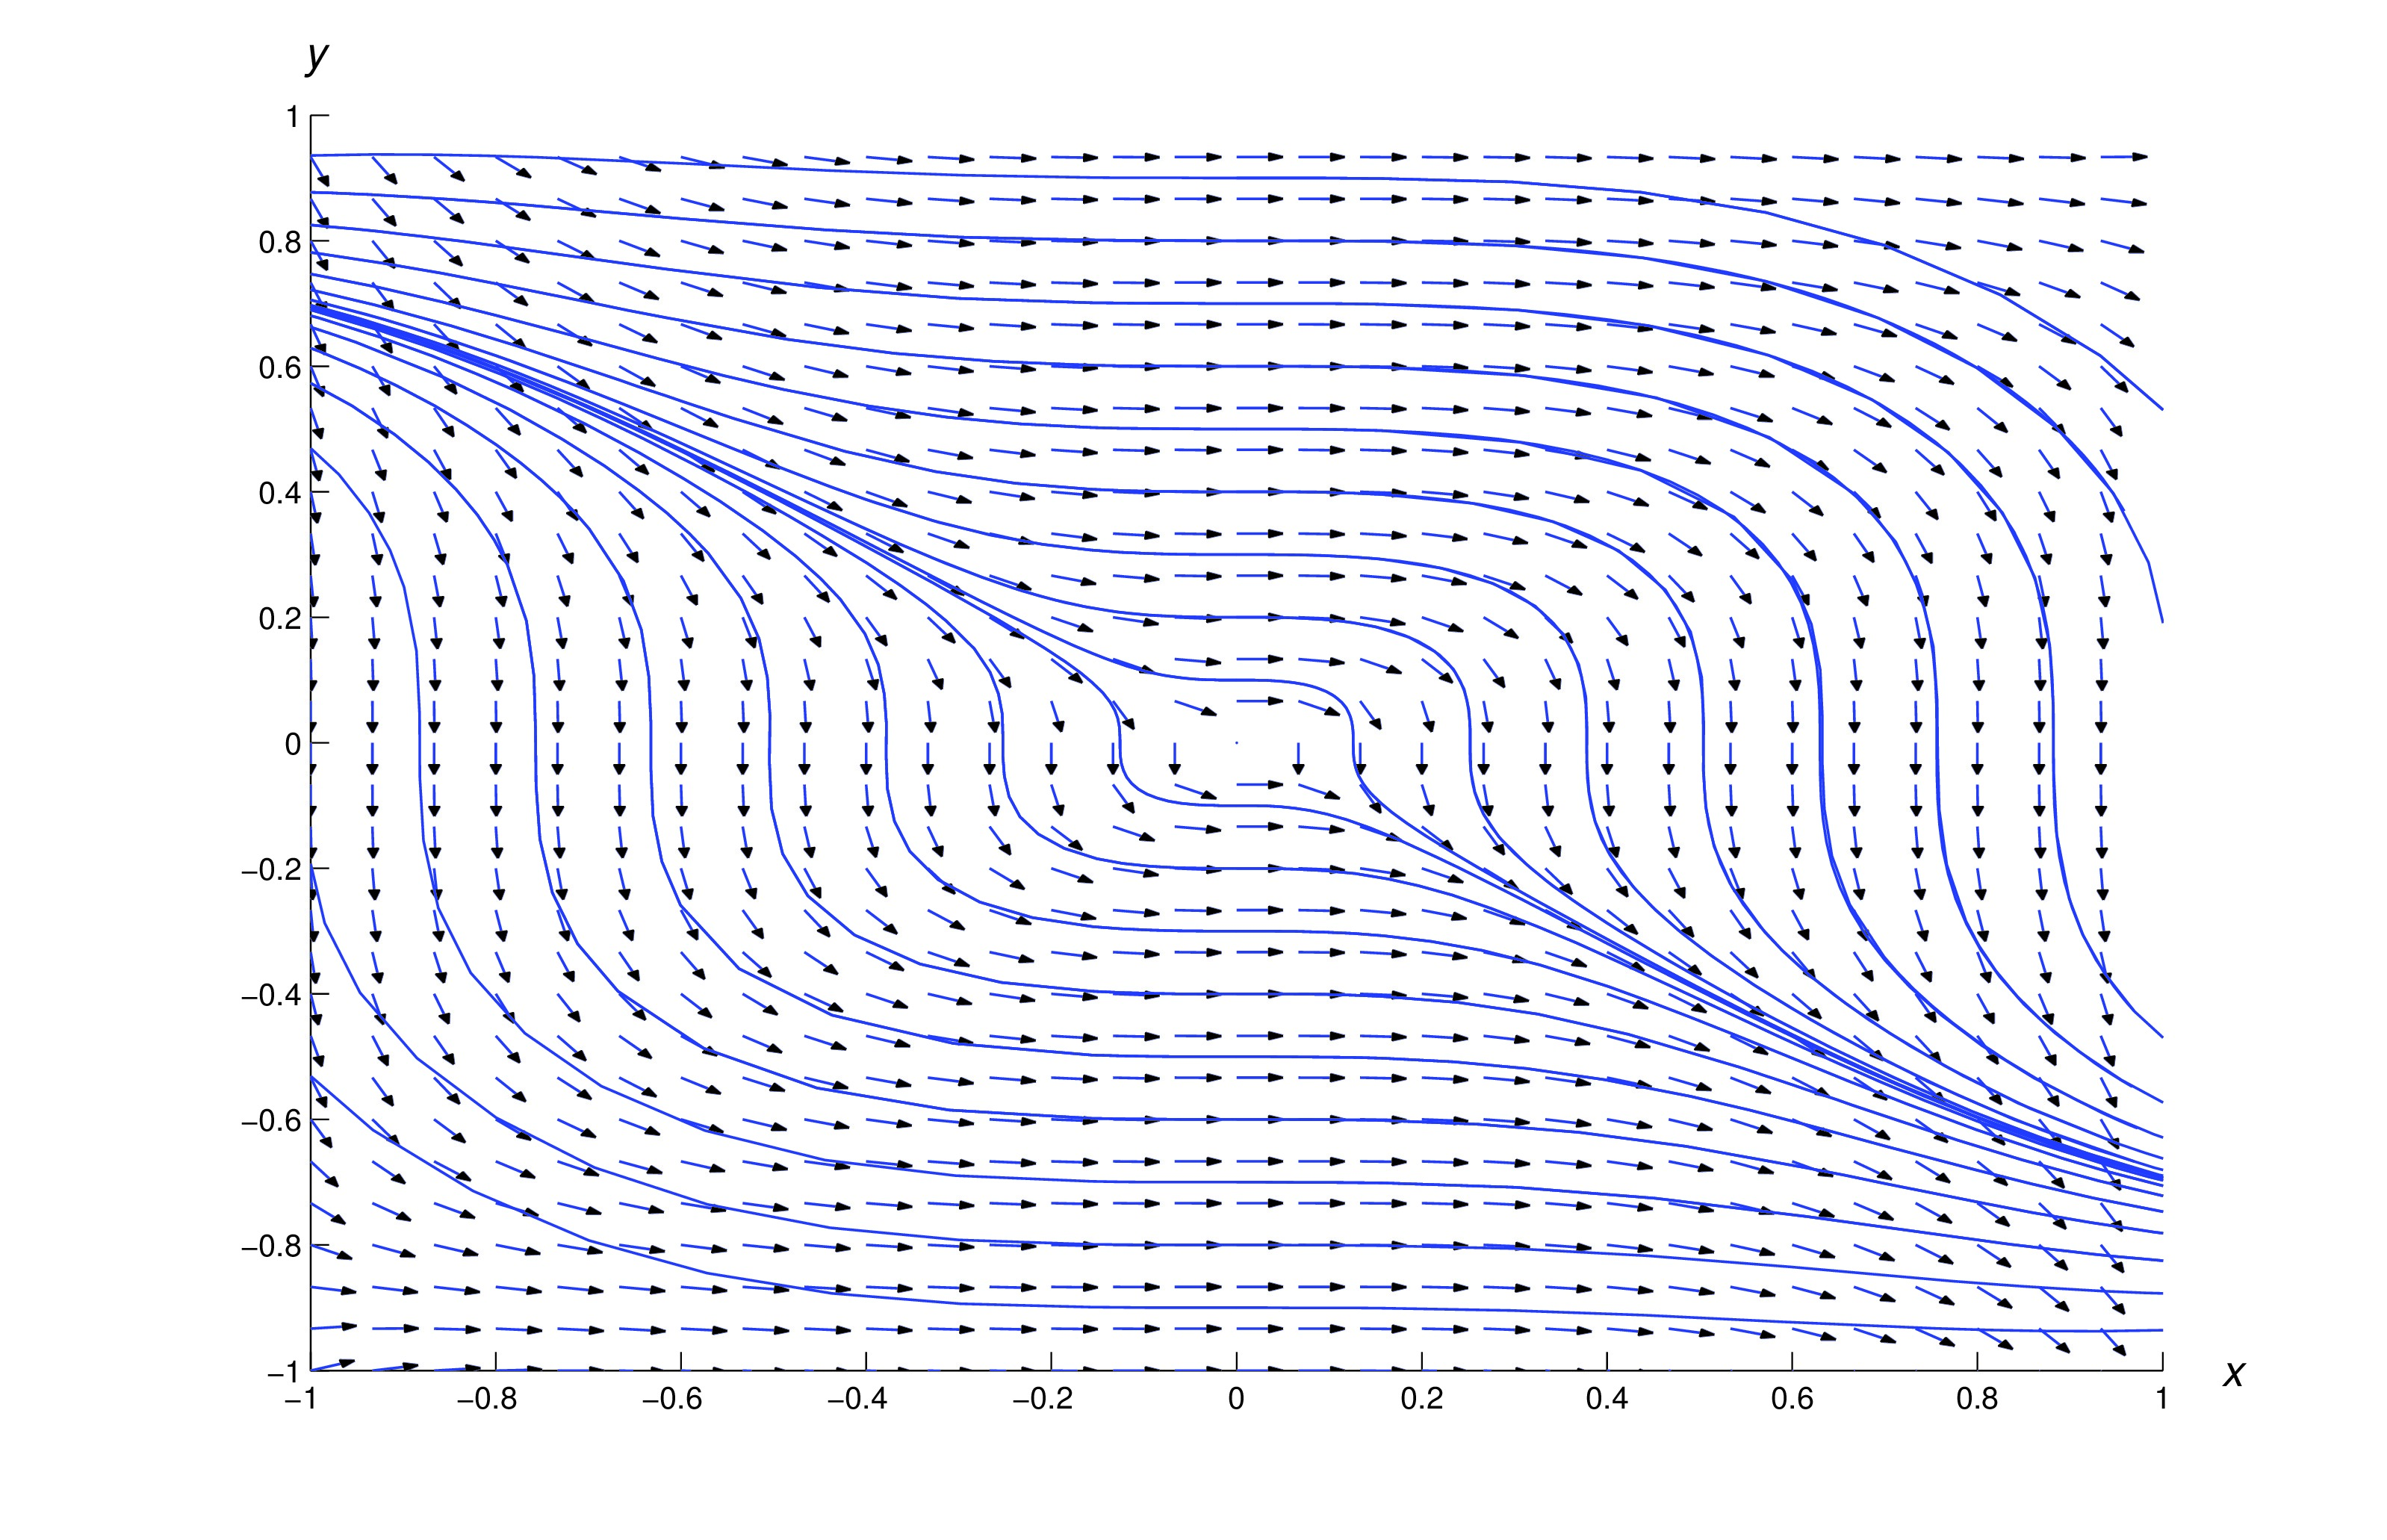
\includegraphics[height=1.5in]{fig020501.jpg} \end{image}
\begin{center}
\begin{figure}
   \caption{A direction field and  integral curves for
$(4x^3y^3+3x^2)\,dx+(3x^4y^2+6y^2)\,dy=0$}
  \label{figure:2.5.1}
\end{figure}
\end{center}
\end{explanation}
\end{example}


Here's a summary of the procedure used in Method 1 of this
example. You should summarize procedure used in Method~2.


Procedure For Solving An Exact
Equation


\begin{procedure}\label{proc:solvingExactEq}

\textit{Step 1.} Check that the equation
\begin{equation} \label{eq:2.5.19}
 M(x,y)\,dx+N(x,y)\,dy=0
\end{equation}
satisfies the exactness condition  $M_y=N_x$. If not,
don't go further with this procedure.

\textit{Step 2.} Integrate
$$
\frac{\partial F(x,y)}{\partial x}=M(x,y)
$$
with respect to $x$ to obtain
\begin{equation} \label{eq:2.5.20}
F(x,y)=G(x,y)+\phi(y),
\end{equation}
where $G$ is an antiderivative of $M$ with respect to $x$, and $\phi$
is an unknown function of $y$.

\textit{Step 3.} Differentiate \eqref{eq:2.5.20} with respect to
$y$  to obtain
$$
\frac{\partial F(x,y)}{\partial y}=\frac{\partial G(x,y)}{\partial
y}+\phi'(y).
$$

\textit{Step 4.} Equate the right side of this equation to $N$ and solve
for $\phi'$;    thus,
$$
 \frac{\partial G(x,y)}{\partial y}+\phi'(y)=N(x,y),\quad\text{so}\quad
\phi'(y)=N(x,y)-\frac{\partial G(x,y)}{\partial y}.
$$

\textit{Step 5.} Integrate $\phi'$ with respect to $y$, taking the
constant of integration to be zero, and substitute the result in
\eqref{eq:2.5.20} to obtain $F(x,y)$.

\textit{Step 6.} Set $F(x,y)=c$ to obtain an implicit solution of
\eqref{eq:2.5.19}. If possible, solve for $y$ explicitly as a
function of $x$.

\end{procedure}



It's a common mistake to omit Step 6. However, it's important to
include this step, since $F$ isn't  itself a solution of
\eqref{eq:2.5.19}.

Many equations can be conveniently solved by either of the two methods
used in Example~\ref{example:2.5.3}. However, sometimes the integration
required in one approach is  more difficult than in the
other. In such cases we choose the approach that requires the easier integration.

\begin{example}\label{example:2.5.4}
 Solve the equation
\begin{equation}  \label{eq:2.5.21}
(ye^{xy} \tan x+e^{xy} \sec^2x)\,dx+xe^{xy} \tan x\,dy=0.
\end{equation}


\begin{explanation} We leave it to you to check that
$M_y=N_x$ on any open rectangle  where $\tan x$ and $\sec x$ are
defined. Here we must find a function $F$ such that
\begin{equation} \label{eq:2.5.22}
F_x(x,y)=ye^{xy} \tan x+e^{xy} \sec^2 x
\end{equation}
 and
\begin{equation}  \label{eq:2.5.23}
F_y(x,y)=xe^{xy} \tan x.
\end{equation}
 It's difficult to integrate \eqref{eq:2.5.22} with respect to $x$, but
easy to integrate \eqref{eq:2.5.23} with respect to $y$.  This yields
\begin{equation} \label{eq:2.5.24}
F(x,y)=e^{xy} \tan x+\psi (x).
\end{equation}
Differentiating this with respect to $x$ yields
$$
F_x(x,y)=ye^{xy}\tan x+e^{xy}\sec^2x+\psi'(x).
$$
 Comparing this with \eqref{eq:2.5.22} shows that  $\psi'(x)=0$.
Hence, $\psi$ is  a constant, which we can take to be zero in
\eqref{eq:2.5.24}, and
$$
e^{xy} \tan x=c
$$
is an implicit solution of \eqref{eq:2.5.21}.
\end{explanation}
\end{example}

Attempting to apply our procedure to an equation that isn't  exact
will lead to failure in  Step 4, since the function
$$
 N-\frac{\partial G}{\partial y}
$$
won't be independent of $x$ if $M_y\neq N_x$,
%(Exercise~\ref{exer:2.5.31})
and therefore
can't be the derivative of a function of $y$ alone. Here's an example that
illustrates this.

\begin{example}\label{example:2.5.5}
 Verify that the equation
\begin{equation} \label{eq:2.5.25}
3x^2y^2\,dx+6x^3y\,dy=0
\end{equation}
is not exact, and show  that the procedure for solving exact equations
  fails when applied to \eqref{eq:2.5.25}.


\begin{explanation}   Here
$$
M_y(x,y)=6x^2y\quad \text{and}\quad N_x(x,y)=18x^2y,
$$
so \eqref{eq:2.5.25} isn't  exact. Nevertheless,  let's try to find
a function $F$ such that
\begin{equation} \label{eq:2.5.26}
F_x(x,y)=3x^2y^2
\end{equation}
and
\begin{equation} \label{eq:2.5.27}
F_y(x,y)=6x^3y.
\end{equation}
Integrating \eqref{eq:2.5.26} with respect to $x$ yields
$$
F(x,y)=x^{\answer{3}}y^{\answer{2}}+\phi(y),
$$
and differentiating this with respect to $y$ yields
$$
F_y(x,y)=\answer{2}x^{\answer{3}}y+\phi'(y).
$$
For this equation to be consistent with \eqref{eq:2.5.27},
$$
6x^3y=2x^3y+\phi'(y),
$$
or
$$
\phi'(y)=4x^3y.
$$
This is a contradiction, since $\phi'$  must be independent
of $x$. Therefore the procedure fails.
\end{explanation}
\end{example}




\section*{Text Source}
Trench, William F., "Elementary Differential Equations" (2013). Faculty Authored and Edited Books \& CDs. 8. (CC-BY-NC-SA)

\href{https://digitalcommons.trinity.edu/mono/8/}{https://digitalcommons.trinity.edu/mono/8/}

\end{document}